% !TEX root = ../main.tex
%-----------------------------------------------------------------------
%  Title block, the problem, the idea, and the training/use flowchart.
%  \input by ../main.tex -- not compiled on its own.
%-----------------------------------------------------------------------
\begin{center}
{\large\bfseries Concept Note: A Neural-Network Surrogate for Ocean Adjoint Sensitivities}\\[2pt]
{\small Tanvir Shahriar \quad$\cdot$\quad DINO configuration, MITgcm
 \quad$\cdot$\quad \today}
\end{center}

\hd{The problem, and the idea.}
The adjoint gives us the sensitivity of the overturning volume transport to everything we
declare as a control --- initial state, surface forcing, mixing parameters --- in a single
backward integration. What it returns, however, is a derivative evaluated at one state and
one set of parameter values, so strictly every setting calls for a run of its own, and each
run is five model years of adjoint integration --- about a day on 27 processors, in the
configuration of the reference run, a completed five-year adjoint. We would like to know
whether, and how, sensitivity varies across a few hundred parameter settings, and at that
price the adjoint alone cannot get us there. The alternative is to train a network to
reproduce what the adjoint would have returned, and to consult it in place of a further
backward integration. This is a supervised learning problem: the adjoint runs completed so
far already have the form of training examples, each associating an ocean state and a
parameter setting with the sensitivity fields the adjoint produced, and it is those fields
the network would learn to predict. The runs are too few to train on, however, and they vary
one factor at a time, so constructing a suitable training set is itself an open question.
Building that set would still require the adjoint, but the cost would be incurred once, in
advance, rather than at every parameter setting. What follows is a first sketch of how such
a surrogate might be posed.

\vspace{3pt}
\begin{center}
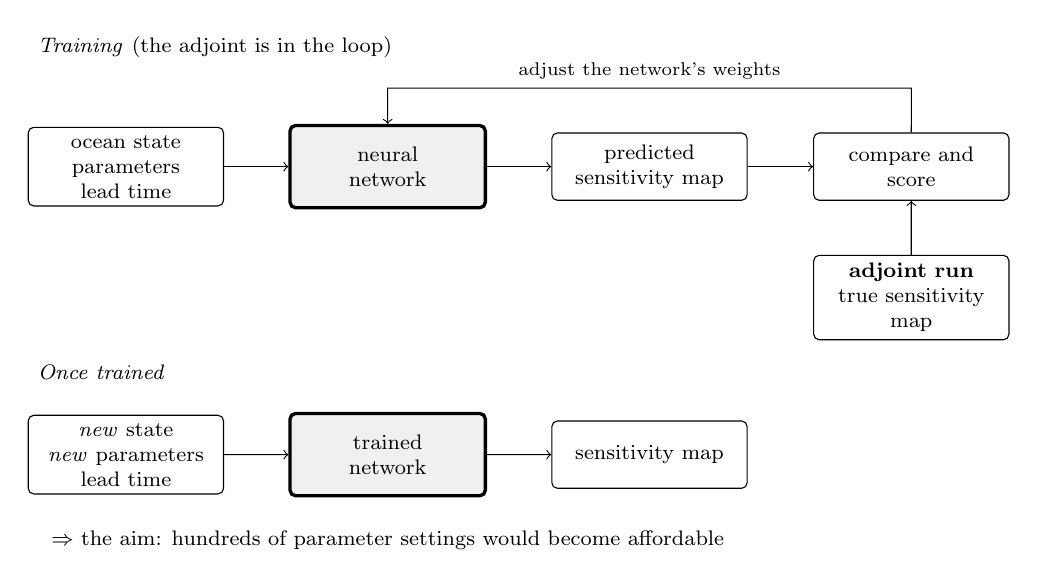
\begin{tikzpicture}[scale=0.95, transform shape,
  font=\footnotesize,
  box/.style={draw, rounded corners=2pt, align=center, inner sep=3pt,
              text width=24mm, minimum height=9mm},
  net/.style={draw, very thick, rounded corners=2pt, align=center, inner sep=3pt,
              text width=24mm, minimum height=11mm, fill=black!6},
  lbl/.style={font=\footnotesize\itshape}]

\node[lbl, anchor=west] at (-1.3,1.6) {Training \textnormal{(the adjoint is in the loop)}};
\node[box] (in)   at (0,0)      {ocean state\\ parameters\\ lead time};
\node[net] (nn)   at (3.5,0)    {neural\\ network};
\node[box] (pred) at (7.0,0)    {predicted\\ sensitivity map};
\node[box] (score) at (10.5,0)  {compare and\\ score};
\node[box] (true) at (10.5,-1.75){\textbf{adjoint run}\\ true sensitivity\\ map};
\draw[->] (in) -- (nn);
\draw[->] (nn) -- (pred);
\draw[->] (pred) -- (score);
\draw[->] (true) -- (score);
\draw[->] (score.north) -- (10.5,1.05) --
      node[above, font=\scriptsize] {adjust the network's weights} (3.5,1.05) -- (nn.north);

\node[lbl, anchor=west] at (-1.3,-2.75) {Once trained};
\node[box] (in2)  at (0,-3.85)   {\emph{new} state\\ \emph{new} parameters\\ lead time};
\node[net] (nn2)  at (3.5,-3.85) {trained\\ network};
\node[box] (out2) at (7.0,-3.85) {sensitivity map};
\draw[->] (in2) -- (nn2);
\draw[->] (nn2) -- (out2);
\node[lbl, anchor=north] at (3.5,-4.75)
     {\textnormal{$\Rightarrow$ the aim: hundreds of parameter settings would become affordable}};
\end{tikzpicture}
\end{center}
